\chapter{Introduction} \label{introduction}

\section{Nuclear Power} % Complete

In the summer of 1956, the world's first commercial nuclear power plant was connected to the grid in the north of England. This marked a significant departure from previous forms of commercial energy production, which relied on relatively low energy density sources such as combustion of coal, oil and gas. Before this, the closest anyone had come to utilising nuclear energy commercially was through geothermal power, where the thermal energy input is partly due to radiogenic heat from unstable isotopes in the Earth's mantle \cite{gando2011partial}. 
%which relied on the chemical reactions of coal oil and gas
%Combustion is a chemical process, where energy differences between reactants and products are exploited via electron exchange. Nuclear energy however, exploits the energy difference between nuclei. Both rely on the conversion of mass into energy, however, the amount of energy that can be extracted varies by several orders of magnitude

Combustion is a chemical process whereby energy differences between reactants and products are exploited via electron exchange. Nuclear energy exploits the energy difference between nuclei. Both rely on the conversion of mass into energy, however, the amount of energy that can be extracted from the nucleus is several orders of magnitude greater.
%Combustion is a chemical process, and its use in commercial energy production is fundamentally about exploiting the free energy difference when electrons are exchanged between some reactants to produce some products. Nuclear energy, however, is about the direct conversion of mass into energy. The difference between the two is staggering.

Consider methane, with an enthalpy of combustion of −887.2 kJ/mol \cite{thornton1917xv}. This is the equivalent of 9.14 eV per particle. By comparison, the total energy release from fission of one uranium-235 nucleus is at least $1.65 \times 10^{8}$ eV, as shown in Figure \ref{figure:fissionenergy}.

Combustion-based power as a technology has matured over hundreds of years, with modern optimisations only looking to offer fractional percent gains in efficiency. By comparison, nuclear power technology is far from mature, with large improvements yet to be realised. One such feature is load-following, an enormously useful feature for a power plant which is currently underutilised in nuclear reactors. Load-following, as currently practiced in some French and German nuclear power plants, is defined as operation where power output follows a variable load programme on a daily basis with several power changes (i.e. to follow the change in electricity demand over a 24 hour period). These power variations can be as large as 50\% of a reactor's rated power \cite{lokhov2011technical}. The biggest obstacle to load-following in nuclear reactors is the issue of pellet-cladding interaction (PCI), which is the basis of the work in this thesis.

\begin{figure}[ht]
\centering
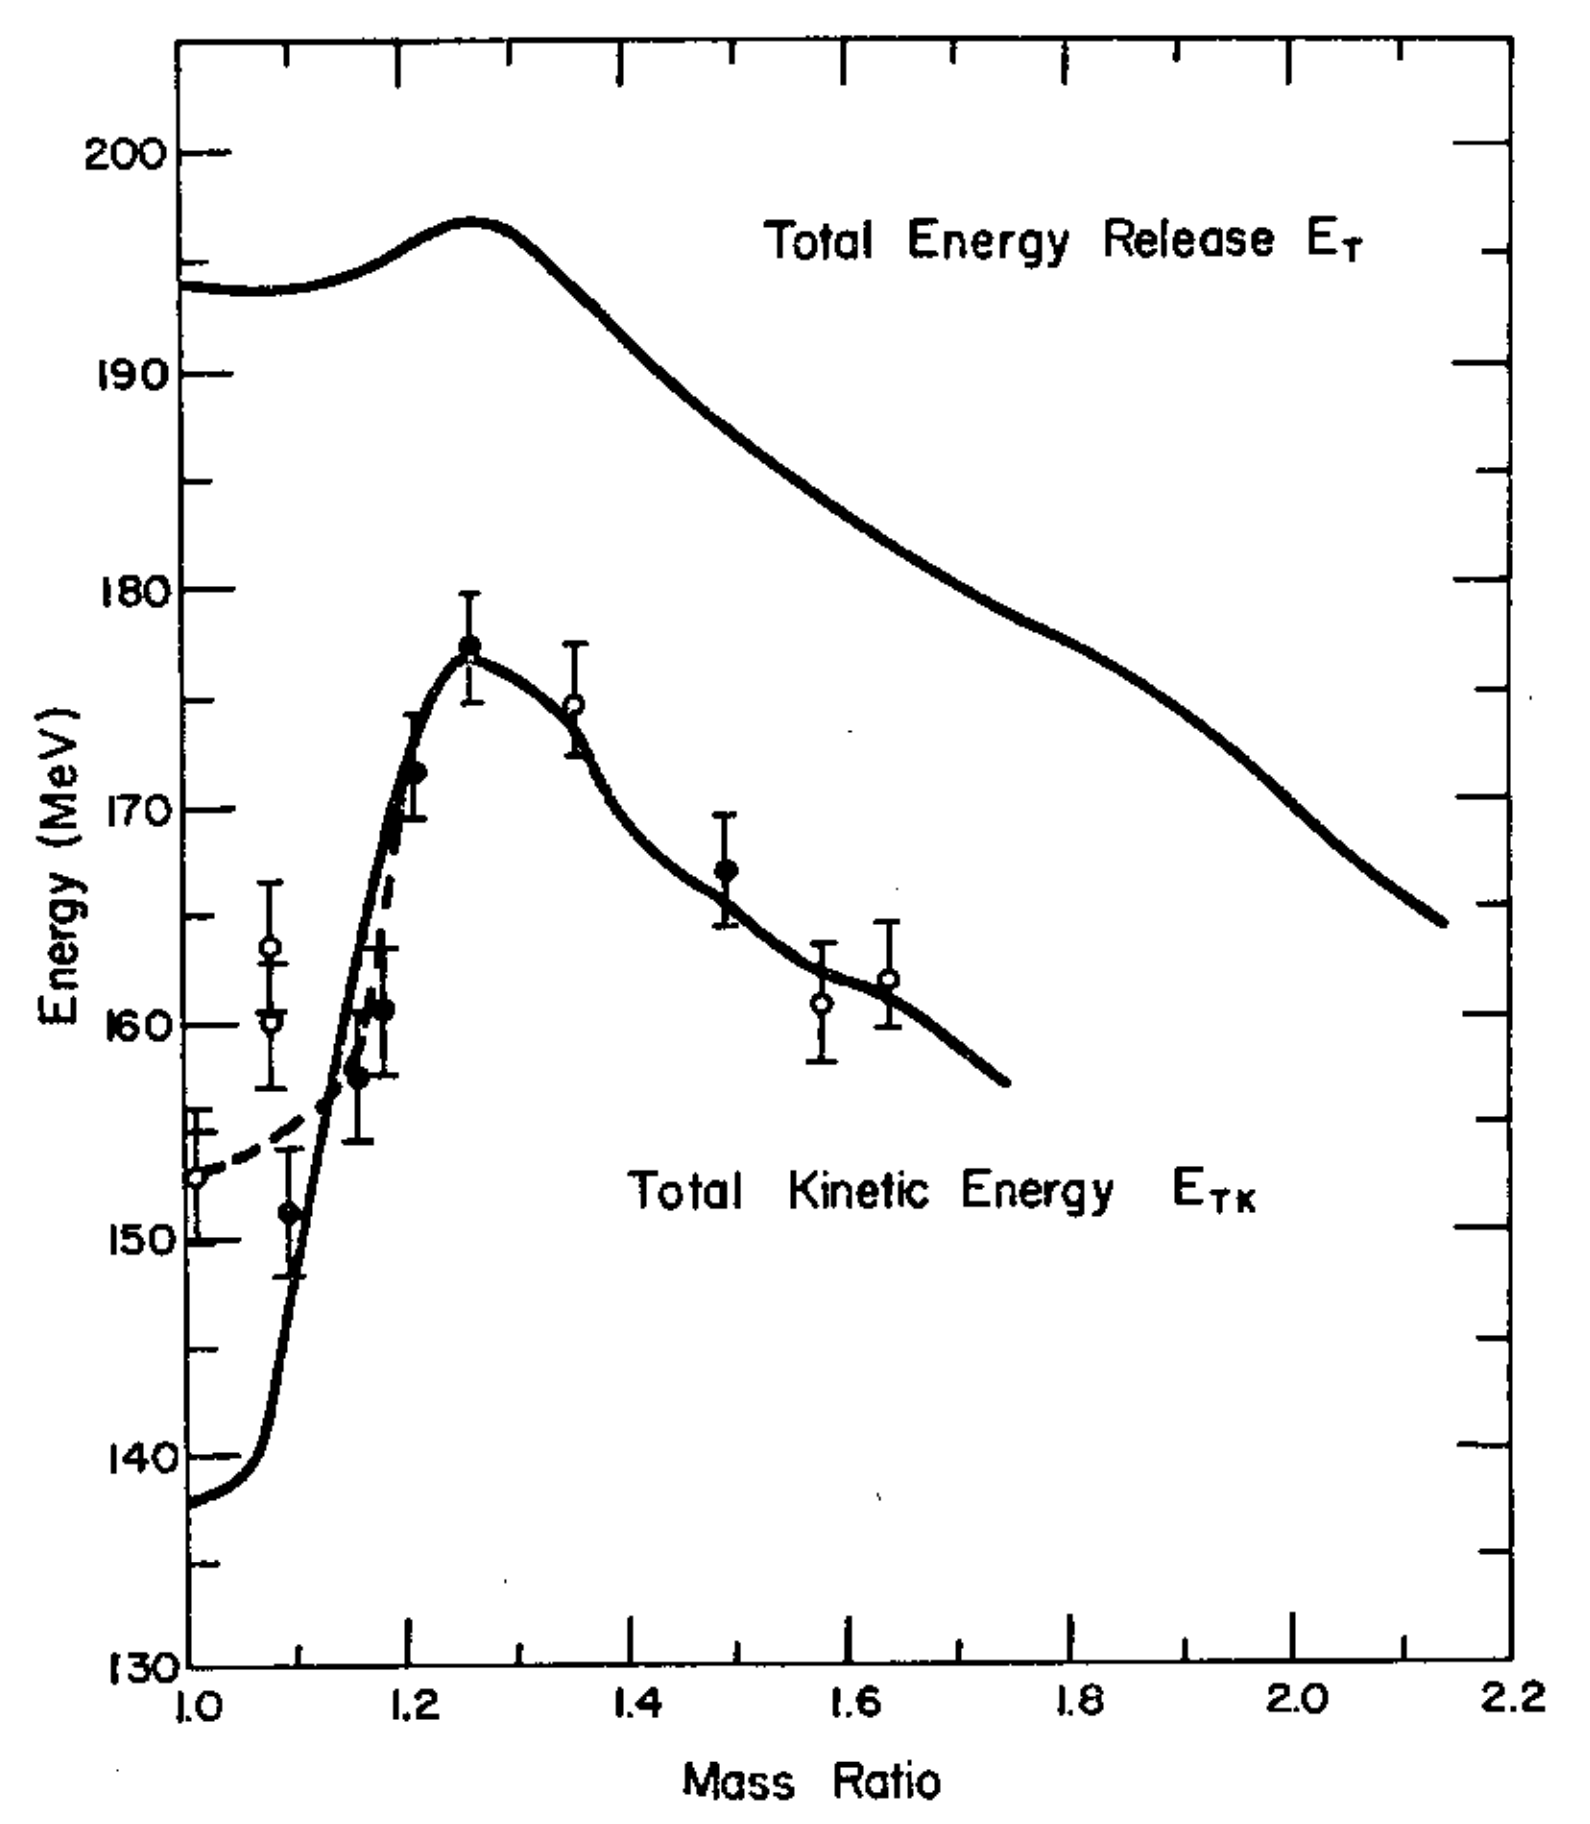
\includegraphics[height=13cm]{images/fission_energy_total.png}
\caption[Energy from thermal fission of U-235 as a function of mass ratios of daughter nuclei. Total energy release includes contributions from gamma rays and subsequent radioactive decays.]{Energy from thermal fission of U-235 as a function of mass ratios of daughter nuclei. Total energy release includes contributions from gamma rays and subsequent radioactive decays. Taken from \cite{aras1965ranges}.}
\label{figure:fissionenergy}
\end{figure}

\subsection{Fission}

Commercial nuclear power plants extract energy through the process of fission, where a large nucleus is split into smaller nuclei. While it is also possible to extract energy from certain small nuclei by the process of fusing them into larger ones, no fusion reactor currently exists which achieves a net positive energy output. At a fundamental level, both fission and fusion rely upon mass-energy equivalence. The relationship between mass and energy is shown using Einstein's equation:
\begin{equation}
\label{emc2}
    E = mc^{2}
\end{equation}
where $E$ is the energy of the system, $m$ is the mass and $c$ is the speed of light. Using this equation we can analyse a typical fission reaction:
\begin{equation}
    \ch{U^{235}_{92}} + n^{1}_{0} \xrightarrow[]{absorption} \ch{U^{236}_{92}} \xrightarrow[]{fission} \ch{I^{132}_{53}} + \ch{Y^{101}_{39}} + 3n^{1}_{0}
\label{eqn:fission} 
\end{equation}
While the number of protons and neutrons are conserved throughout the reaction, a mass difference calculation will show that there is actually less mass in the products than the reactants by approximately 0.188 amu (3.127$\times 10^{-28}$ kg). This missing mass, known as the \emph{mass defect}, is converted to energy ($\sim$175 MeV). In this way, the total mass-energy of the system is conserved. Some of this energy is carried away as kinetic energy of the fission products (in Equation \ref{eqn:fission}, I and Y) and also the kinetic energy of the neutrons. The neutrons at this stage have energies \goodtilde{1} MeV and are known as \emph{fast} neutrons.

This change in mass arises due to the phenomenon of \emph{binding energy}. In order for two or more nucleons to be thermodynamically stable when bound together, the total free energy of the bound configuration must be less than the sum of constituent nucleon free energies. Much as with energy stored in a chemical bond, the binding energy represents the energy required to separate the nucleus into individual protons and neutrons. 

Larger nuclei will generally have a greater total binding energy value compared to smaller nuclei, but the mass defect per nucleon will not necessarily be the same in a larger nucleus. It is therefore useful to normalise the binding energy by the mass number. Different isotopes have different binding energies, and any nuclear reaction that increases the binding energy per nucleon will be exothermic, whether by fission or fusion. Figure \ref{figure:bindingenergy} shows a plot of binding energy per nucleon against mass number with the relevant isotopes from Equation \ref{eqn:fission}. 

%235.0439299 + 1.008664 (236.0525939) -> 131.907997 + 100.93031 + 3.025992 (235.864299)
\begin{figure}[ht]
\centering
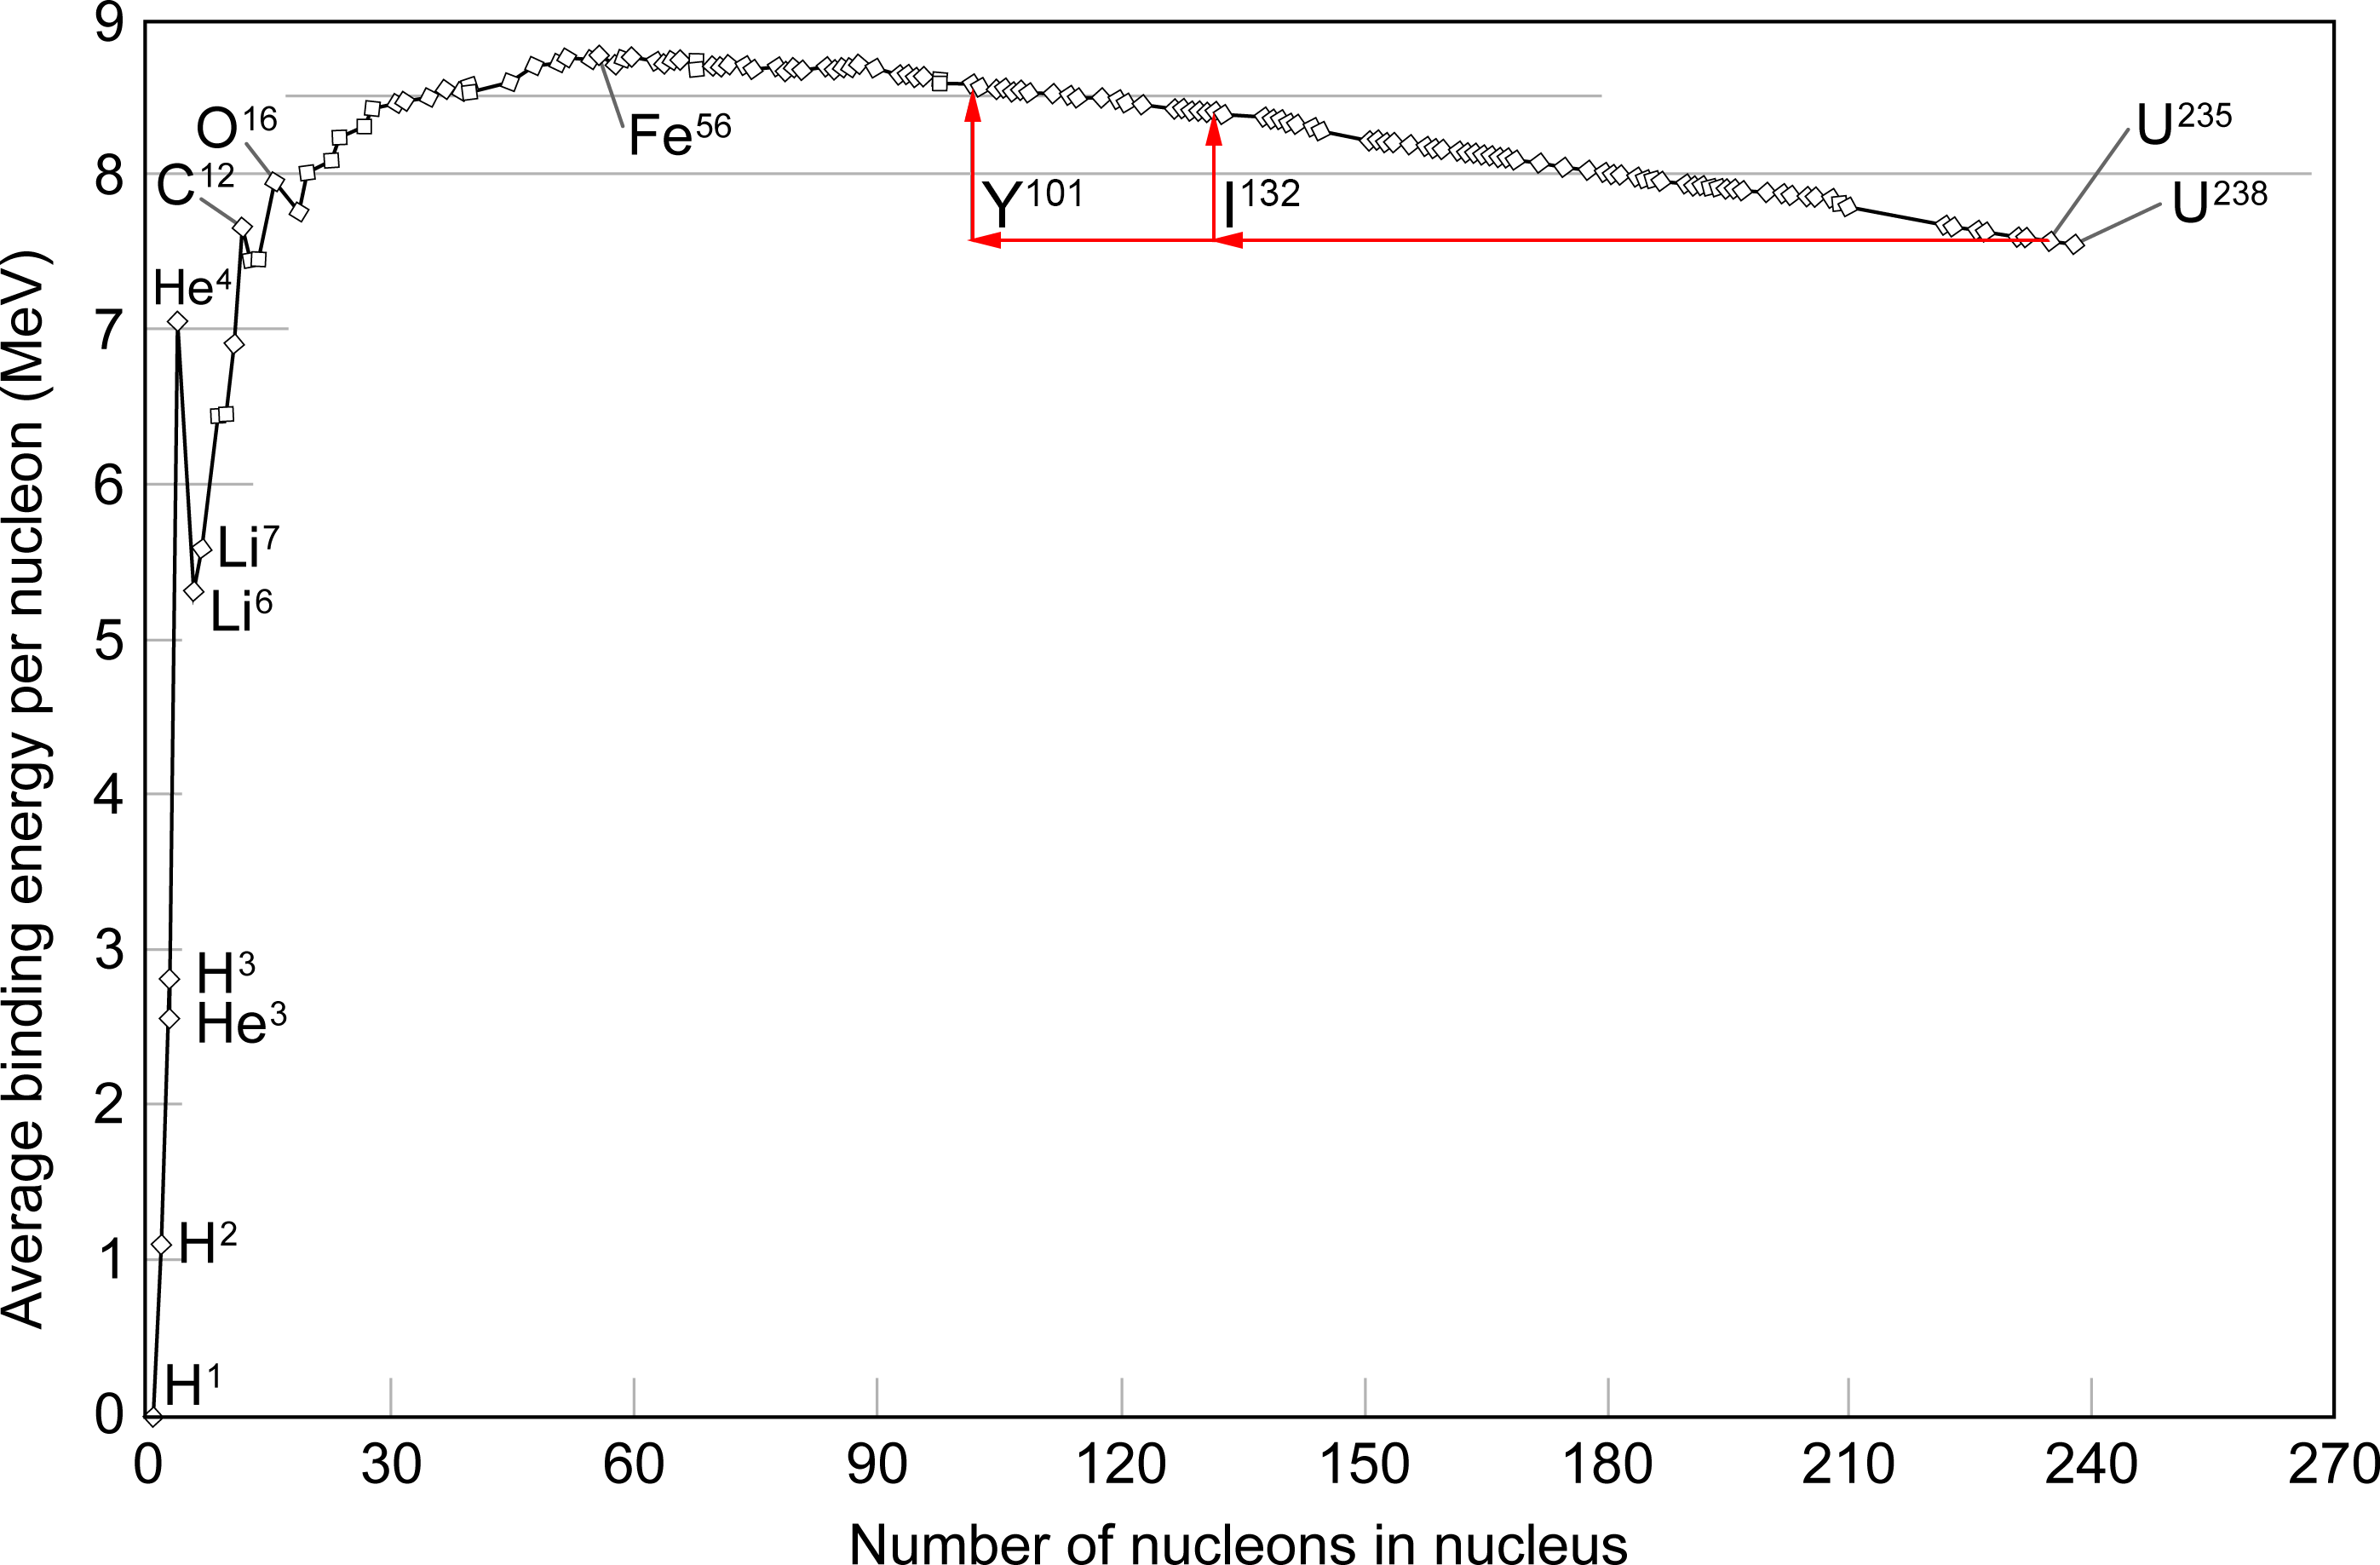
\includegraphics[width=14cm]{images/Binding_energy_curve.png}
\caption[Plot binding energy per nucleon against mass number. Arrows indicate the reaction shown in equation \ref{eqn:fission}.]{Plot binding energy per nucleon against mass number. Arrows indicate the reaction shown in equation \ref{eqn:fission}. Adapted from \cite{Fastfission}.}
\label{figure:bindingenergy}
\end{figure}

\subsection{Reactor design} % Complete

Commercial nuclear reactors are large boilers in a Rankine cycle, designed to maximise heat transfer to a working fluid. All nuclear plants use steam turbines on the generation side, though the reactor coolant may be another fluid in a separate loop, such as carbon dioxide in gas-cooled reactors (GCRs), or even in a separate water loop such as in pressurised water reactors (PWRs). 

The most prevalent reactor type is the PWR, followed by the boiling water reactor (BWR). Figure \ref{figure:pwrschematic} shows schematically a PWR power plant. This design incorporates a primary coolant loop and heat exchanger to a secondary loop at a lower pressure. Steam is generated on the low pressure side of the heat exchanger which then drives a steam turbine. There are several other reactor types used around the world (enumerated in Table \ref{figure:world_reactors}). The work in this thesis is focused on zirconium-based claddings which are used worldwide in all commercial reactors except GCRs and sodium-cooled fast reactors. In total, zirconium fuel cladding is used in over 95\% of all nuclear reactor fuel pins, and so performance improvements in these cladding materials have an effect across the entire industry.

\begin{figure}[ht] % Schematic of a PWR
\centering
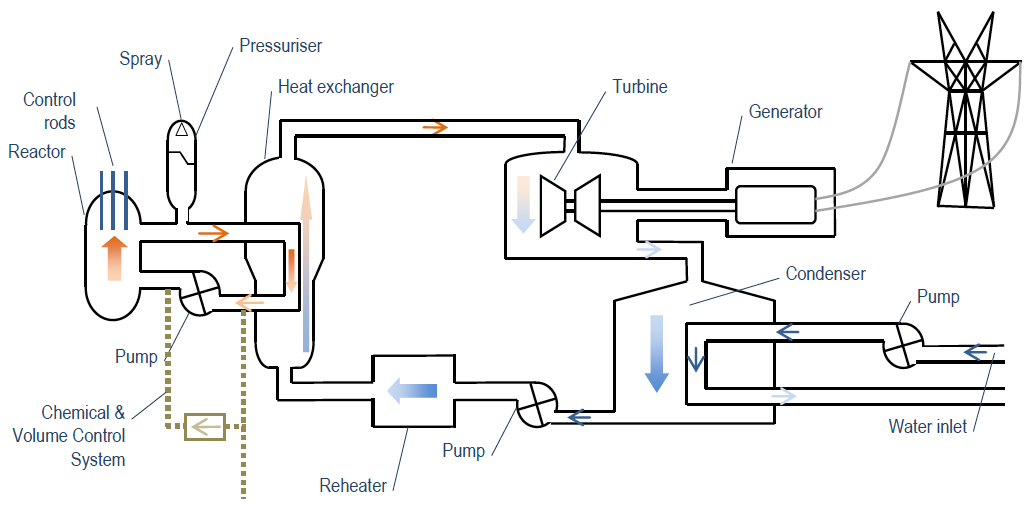
\includegraphics[width=\linewidth]{images/pwrschematic.png}
\caption[Schematic illustration of a PWR power plant.]{Schematic illustration of a PWR power plant. Taken from \cite{lokhov2011technical}.}
\label{figure:pwrschematic}
\end{figure}

The fission of uranium takes place inside a steel reactor pressure vessel (RPV) in PWRs and BWRs, which holds the fuel pins, control rods and other reactor internals. The working fluid in a nuclear reactor is typically under high pressure, with PWR RPV operating pressures between 150 and 160 bar, while BWRs operate at lower pressures of around 70 bar \cite{kok2016nuclear, Server2010, Durmayaz2001}. The pressure of the coolant acts on the fuel cladding, generating radial and hoop stresses which influence crack formation. 

The operating temperature of the coolant in a typical PWR is approximately 600 K. This is a low temperature relative to the melting points of Zr metal (2128 K) and ZrO$_{2}$ (2988 K). This temperature together with the high pressure is chosen in order to keep the coolant in the liquid phase for safety reasons, though this limits the thermodynamic efficiency of the plant. The highest temperature in a reactor will occur in the nuclear fuel, with PWR fuel pellets reaching centreline temperatures of up to 1673 K \cite{beyer1998review}.

\begin{table}[ht] % Reactors in the world
\centering
\caption[Type and number of different reactors operational worldwide at the end of 2017. Change from 2016 shown in parentheses.]{Type and number of different reactors operational worldwide at the end of 2017. Change from 2016 shown in parentheses. Taken from \cite{WNAreport2018}.}
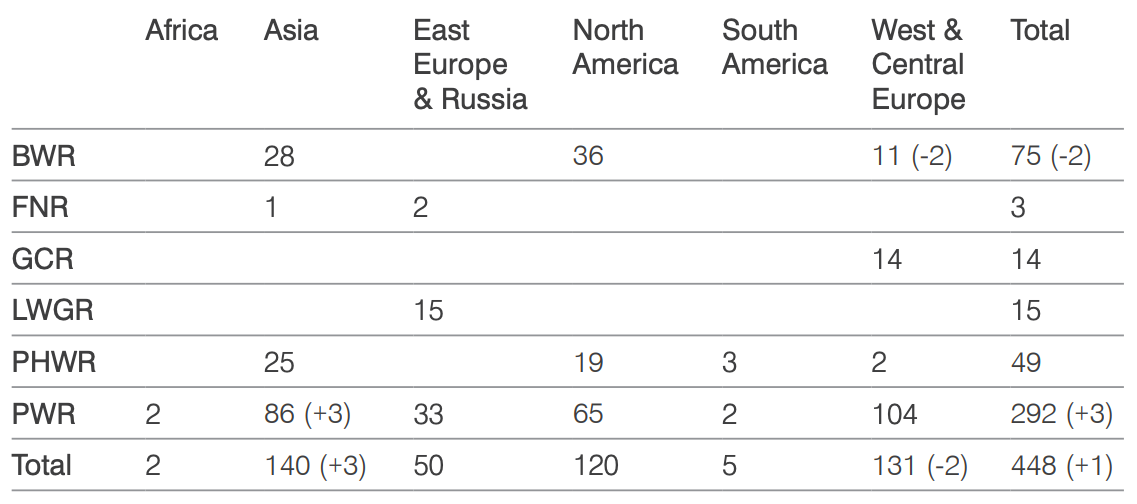
\includegraphics[width=15cm]{images/WNA_report2018.png}
\label{figure:world_reactors}
\end{table}

For both PWRs and BWRs, the coolant is typically light water (as opposed to heavy water, D$_{2}$O). Water is used because it has many useful engineering properties. It has a high heat capacity (compared to the gaseous coolant in gas cooled reactors), has low activation in a free neutron environment and also serves as a good radiation shield. Furthermore, it is plentiful, cheap and easily purified.

In additional to its function as a coolant, water also acts as a neutron moderator, slowing down high-energy fast neutrons from fission events and nuclear decay processes. Moderation of neutrons is an important step in the nuclear reactor because slow thermal neutrons (i.e. neutrons at thermal equilibrium with the coolant) are significantly more likely to cause uranium nuclei to undergo fission than fast neutrons. Fast neutrons will typically escape from the fuel pin after they are generated, dispense most of their energy in the coolant via scattering with H and O nuclei, and then some will re-enter the fuel, where they may cause fission of a U$_{235}$ nucleus near the outer edge of the fuel pellet. Neutrons which do not end up fissioning fuel will either be absorbed parasitically by other nuclei (e.g in the control rods or coolant), escape from the reactor entirely (neutron leakage), or decay into protons (free neutrons have a half-life of 10.61 minutes \cite{Christensen1972}).

\subsection{Fuel pins and cladding} \label{ss_fuelpin}

Fuel assemblies in nuclear reactors are bundles of fuel pins (see Figure \ref{figure:fuelassembly}). In most commercial reactors, fuel pins are comprised of a zirconium-based cladding (tubes), which are filled with cylindrical UO$_{2}$ fuel pellets, each of which are approximately 1 cm$^{3}$ in volume (see Figure \ref{figure:fuelpellet}). Fuel pellets in PWRs and BWRs have dishes on the top and bottom faces of the cylinder as well as chamfered edges. The main function of the dishes is  to reduce the axial pellet-pellet stresses caused due to swelling of the pellet when irradiated \cite{marino2005crack}. Chamfers aid in the loading of fuel pellets into the cladding, as well as reducing the risk of chipping at the edges of the fuel pellet. This is important because chipping of the fuel pellet can lead to debris falling into the pellet-cladding gap where it can act as a stress raiser \cite{doerr2015nuclear}.

\begin{figure}[ht]
\centering
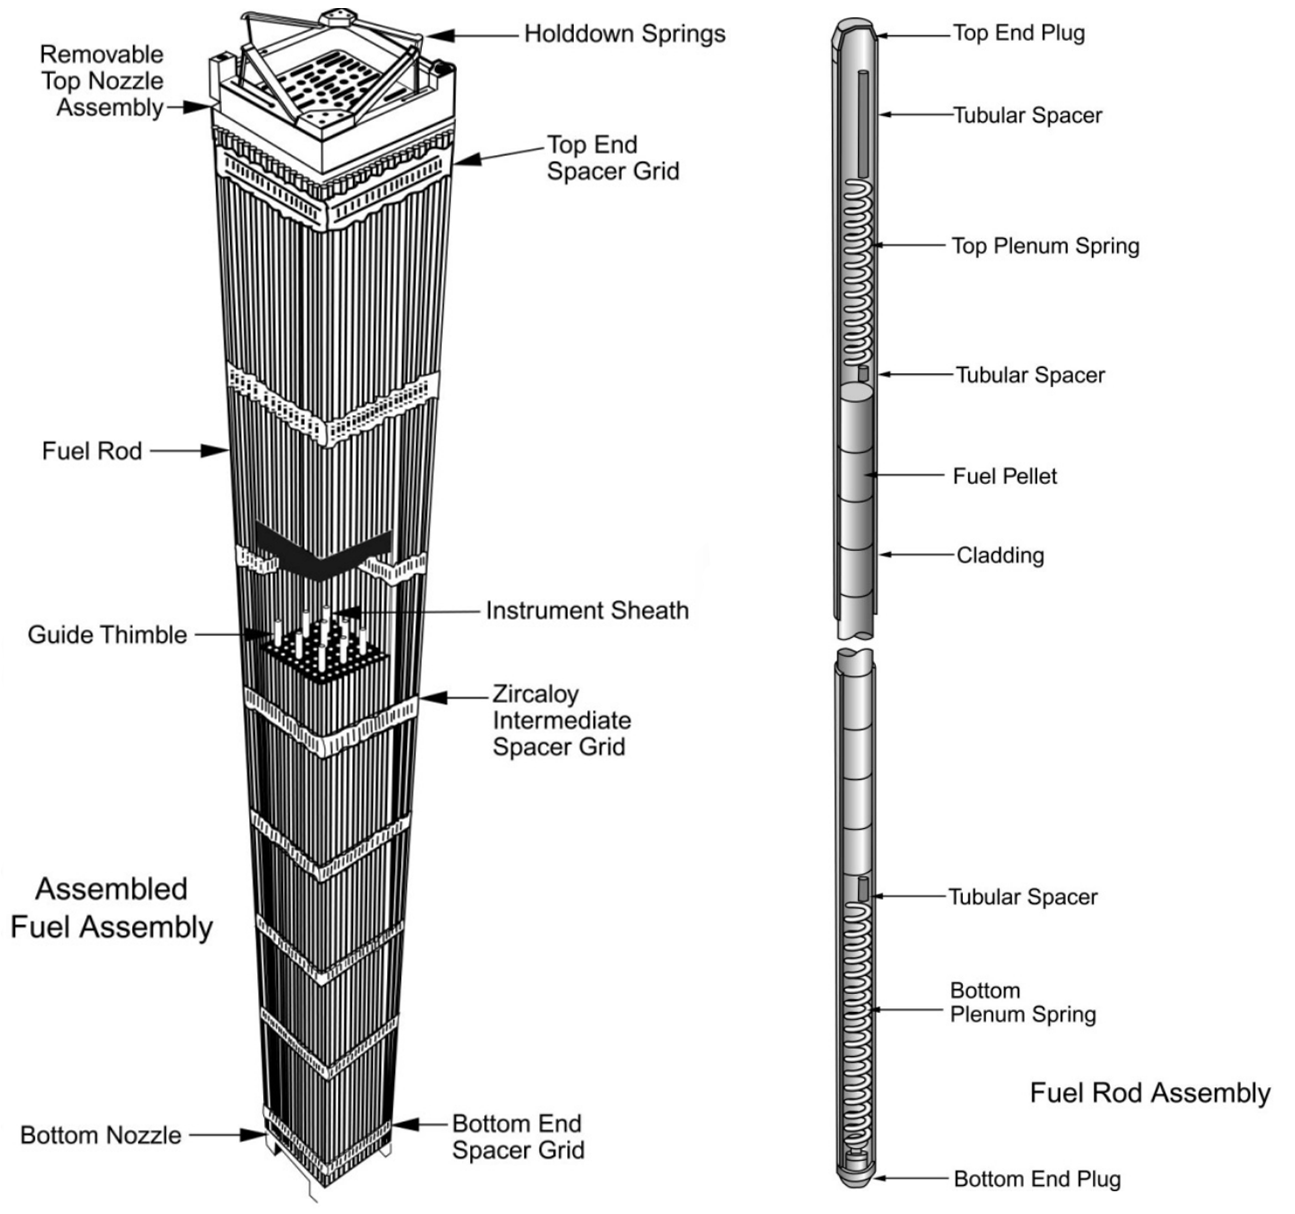
\includegraphics[width=11cm]{images/fuelassembly.png}
\caption[Schematic view of a PWR fuel assembly and a PWR fuel pin.]{Schematic view of a PWR fuel assembly and a PWR fuel pin. Adapted from \cite{Croff2003}.}
\label{figure:fuelassembly}
\end{figure} 

Once loaded with fuel pellets, the fuel pins are capped and filled with inert helium gas, pressurised to between 2 and 25 atm to improve heat transfer from the fuel pellets to the coolant as well as delaying inward creep deformation of the cladding due to the high coolant pressure \cite{King1980}. 

\begin{figure}[ht]
\centering
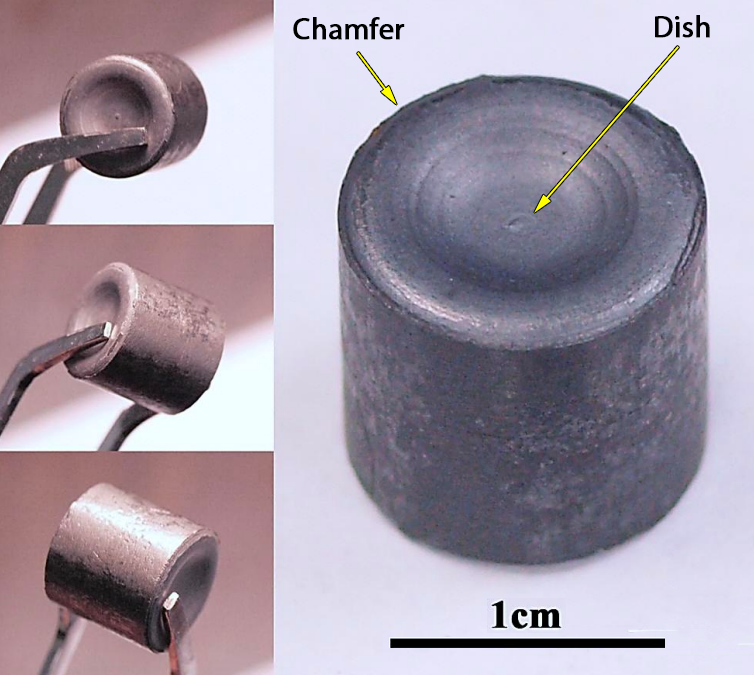
\includegraphics[width=10cm]{images/fuelpellet.png}
\caption[UO$_{2}$ LWR fuel pellet showing dishes and chamfers.]{UO$_{2}$ LWR fuel pellet showing dishes and chamfers. Adapted from \cite{tulenko2013development}.}
\label{figure:fuelpellet}
\end{figure}

In the early stages of a fuel pin's life, there is a small gap between the fuel pellet and the cladding, known as the pellet-cladding gas gap. This gas gap slowly closes with increasing fuel burn-up due to swelling of the fuel pellets and inward creep deformation of the cladding due to the coolant pressure. The pellet-cladding system is shown using a schematic view of the cross section of a PWR fuel pin in Figure \ref{figure:gas_gap}. The cladding internal oxide layer covers the entire internal circumference of the cladding and is the first barrier to corrosive species. 

\begin{figure}[ht]
\centering
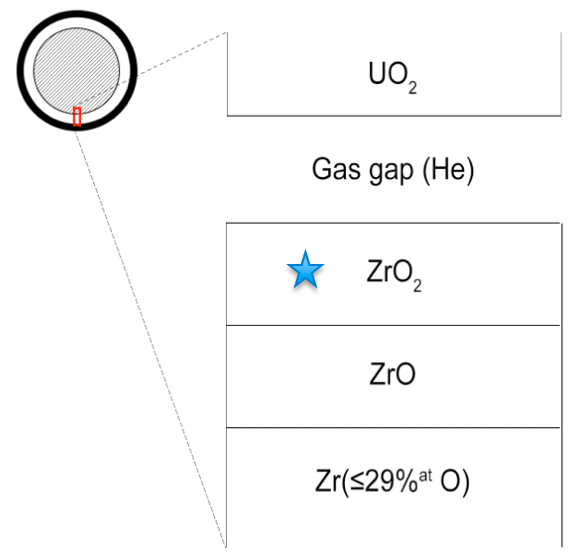
\includegraphics[width=10cm]{images/gas_gap.png}
\caption{Schematic cross-section of a single PWR fuel pin with an expanded view of the pellet-gap-cladding system.}
\label{figure:gas_gap}
\end{figure}

\subsection{Effects of radiation on materials} 

While ionising radiation is always present in the environment as background radiation, the intensity of radiation in a nuclear reactor is so great that it causes significant engineering challenges because of how it affects change in reactor materials.

Radiation hardening (also known as radiation embrittlement) is a phenomenon which affects most materials subjected to ionising radiation. It is characterised by a loss of plasticity caused by radiation damage over time, leading to an increased risk of cracks and failure of components. While zirconium is a very useful nuclear material due to its neutron transparency, it is still susceptible to radiation damage \cite{Wisner1998}. Beyond certain levels of radiation damage, phase changes may also occur. %In \zirconia\ however,  

Amorphisation is another effect of radiation damage, which has been observed in the (Zr, U)O$_{2}$ bonding layer in fuel pins \cite{Nogita1997}. This is characterised by an overall loss of long-range order of atoms in a crystal. This typically occurs beyond a certain threshold of radiation damage depending on the material, called the critical amorphisation dose. Amorphisation is problematic because the loss of a defined crystal structure results in both a reduction in structural stability (amorphous materials have a higher Gibbs free energy than their crystalline counterparts) and causes swelling of the material \cite{Einfal2013}. In the literature, there is evidence of amorphisation in cubic stabilised \zirconia\ when bombarded with Cs$^{+}$ ions up to a fluence of $1 \times 10^{21}$ ions m$^{-2}$ \cite{amorphization2000wang}. However, no amorphisation is seen at an Xe$^{2+}$ fluence of $2 \times 10^{21}$ ions m$^{-2}$, or an I$^{+}$ fluence of $5 \times 10^{19}$ ions m$^{-2}$ \cite{sickafus1999radiation}.

One material phenomenon exclusive to nuclear reactor environments is neutron activation. The high free neutron environment leads to neutron capture in various nuclei within the reactor, including those of the fuel assemblies, coolant and RPV. There are many possible (n, x) reactions that may occur in materials experiencing a neutron flux, but of particular concern is transmutation of nuclei following a nuclear capture event. When a stable nucleus captures a neutron and becomes unstable, the nucleus may then emit particles to reduce its free energy, altering its atomic number in the process. This new element will have different chemical properties compared to the parent nucleus by virtue of a different electronic structure. This will change the elemental composition of a material, typically in an unfavourable way with dopants that negatively affect some desired material property. The extremely large number of nuclei relative to neutron flux means that this effect is small, though over time this becomes more significant due to the accumulation of these dopant elements.

In high-radiation environments, it is also possible for some molecules to be split by gamma photons above certain energies through the process of radiolysis. Corrosive fission products such as iodine will be present inside the fuel pin, but may exist in the form of (for example) CsI, which is not highly corrosive. Radiolysis however, decomposes CsI into Cs and I$_{2}$ vapour which can diffuse towards the cladding and promote cracking \cite{Konashi1983}.

\subsection{Fission products, their distribution and decay chains}

Nuclei which can undergo fission will produce daughter nuclei (fission products) with specific characteristics. At first, these nuclei will almost always be neutron-rich, as compared to their stable isotopes. This is the result of the higher neutron to proton (N/Z) ratios of larger nuclei. Figure \ref{figure:NZcurve} shows how the nuclei of abundant isotopes start with N/Z ratios of around 1 for small elements (e.g. \ch{He_{2}^{4}}, \ch{C_{6}^{12}}, \ch{O_{8}^{16}}), whereas larger elements will have isotopes with N/Z ratios approaching 1.6 (e.g. \ch{Pb_{82}^{208}}, \ch{Th_{90}^{232}}, \ch{U_{92}^{238}}).

\begin{figure}[ht]
\centering
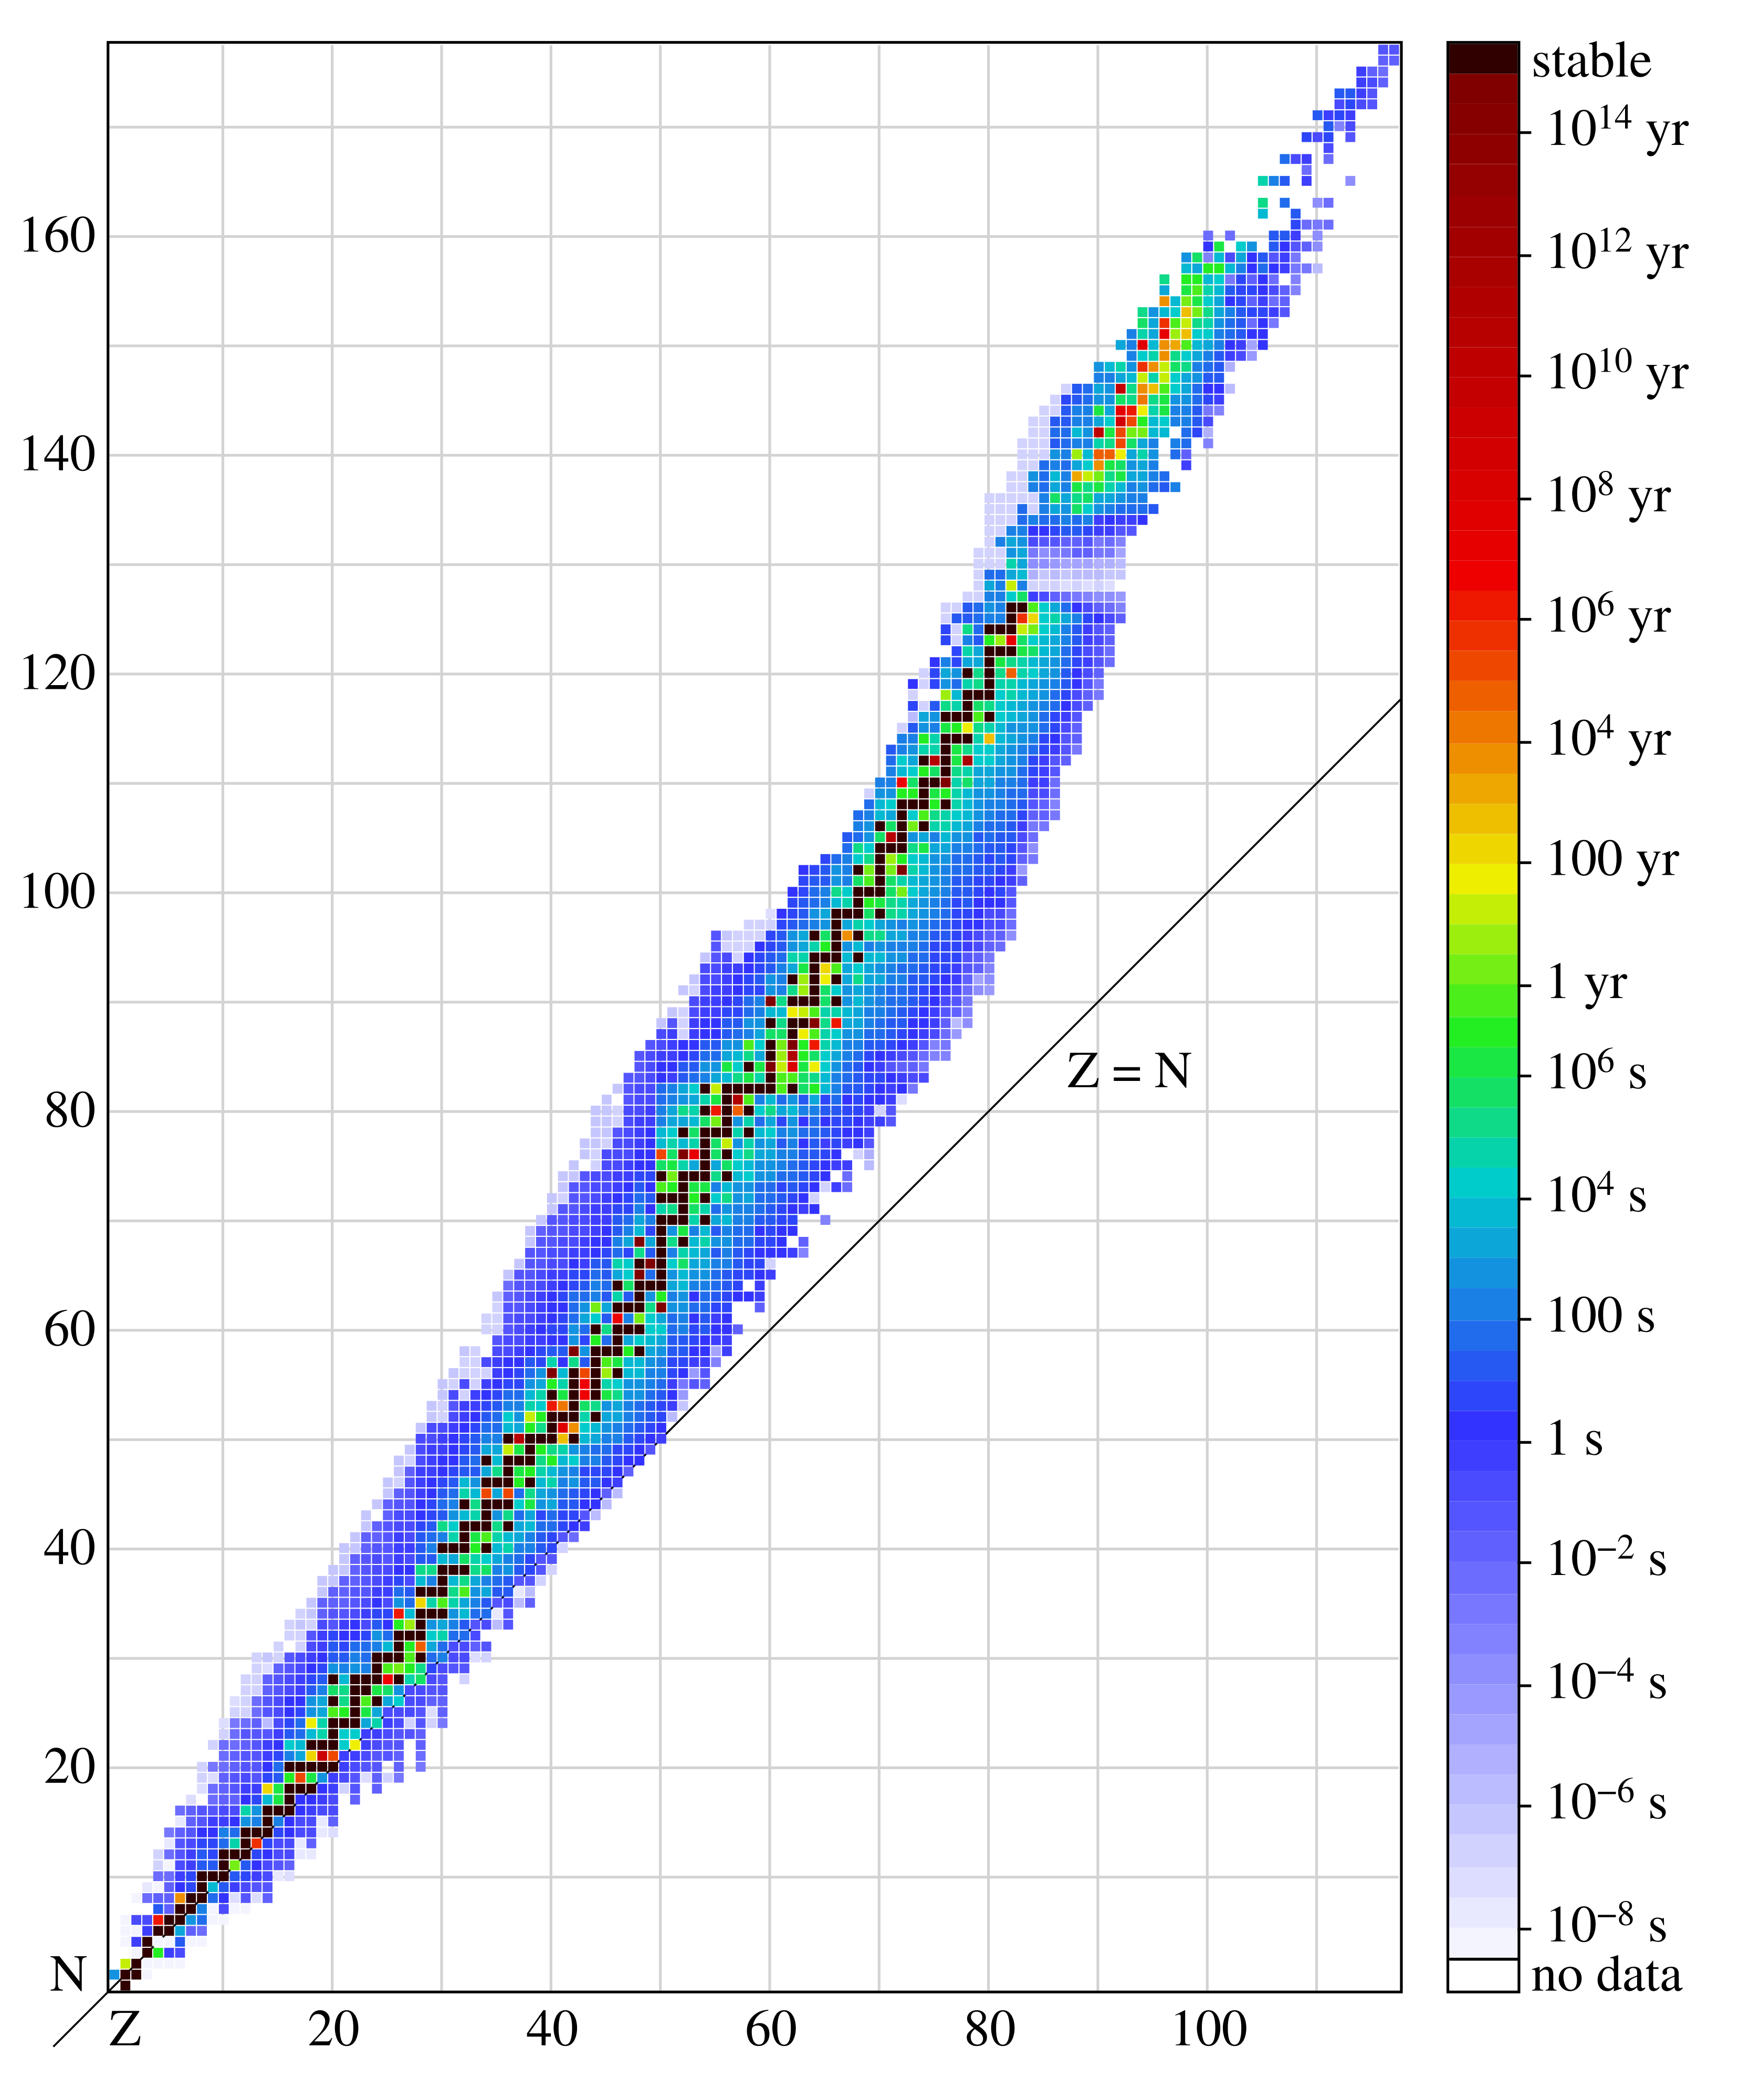
\includegraphics[height=13cm]{images/Isotopes_and_half-life.png}
\caption[Plot of neutron number against proton number for nuclei with half-lives greater than 10${^{-8}}$ s.]{Plot of neutron number against proton number for nuclei with half-lives greater than 10${^{-8}}$ s. Taken from \cite{BenRG}.}
\label{figure:NZcurve}
\end{figure} 

Fissionable nuclei are typically very large and when fission occurs, the daughter nuclei will inevitably inherit a high N/Z ratio. These neutron-rich nuclei will generally decay by $\beta-$ particle emission to reduce their N/Z ratio and increase stability. One decay event is usually not enough to achieve a stable nucleus, so several decays as part of a decay chain are expected. An example is given for Te in Equations \ref{eqn:te_decay} and \ref{eqn:i_decay}.
\begin{gather}
\ch{Te_{134}^{52}} \xrightarrow[]{\beta-} \ch{I_{134}^{53}}+ e^{-} + \overline{\nu}_{e}
\label{eqn:te_decay} \\
\ch{I_{134}^{53}} \xrightarrow[]{\beta-} \ch{Xe_{134}^{54}} + e^{-} + \overline{\nu}_{e}
\label{eqn:i_decay}
\end{gather}
Another characteristic feature of fission products is that their masses are bi-modally distributed. Figure \ref{figure:fissionyield} shows calculated fission yields as a function of mass number, indicating a 40:60 rather than 50:50 mass distribution among daughter nuclei when heavy nuclei are fissioned. This is attributed to smaller nuclei (which have high binding energies per nucleon) separating from the nucleus first at the moment when fission occurs. This results in the majority of fission products centring around atomic masses of 95 and 135, producing a disproportionate number of nuclei such as Sr, Y and Zr on the low side and Te, I and Cs on the high side of the distribution. The distribution of fission products varies slightly depending on which nucleus is fissioned (e.g. U$_{233}$, U$_{235}$, Pu$_{239}$) and the energy of the fissioning neutron. Over time, transmutation of U$_{238}$ to Pu$_{239}$ and consumption of U$_{235}$ means that an increasing proportion of energy output will be due to fission of Pu$_{239}$, but fuel assemblies are typically retired before significant build-up of Pu$_{239}$ inventory and so the net yields of fission products will only change slightly over the life of the fuel.
% Iodine 0.1142684237, Tellurium 0.180582

\begin{figure}[ht!]
\centering
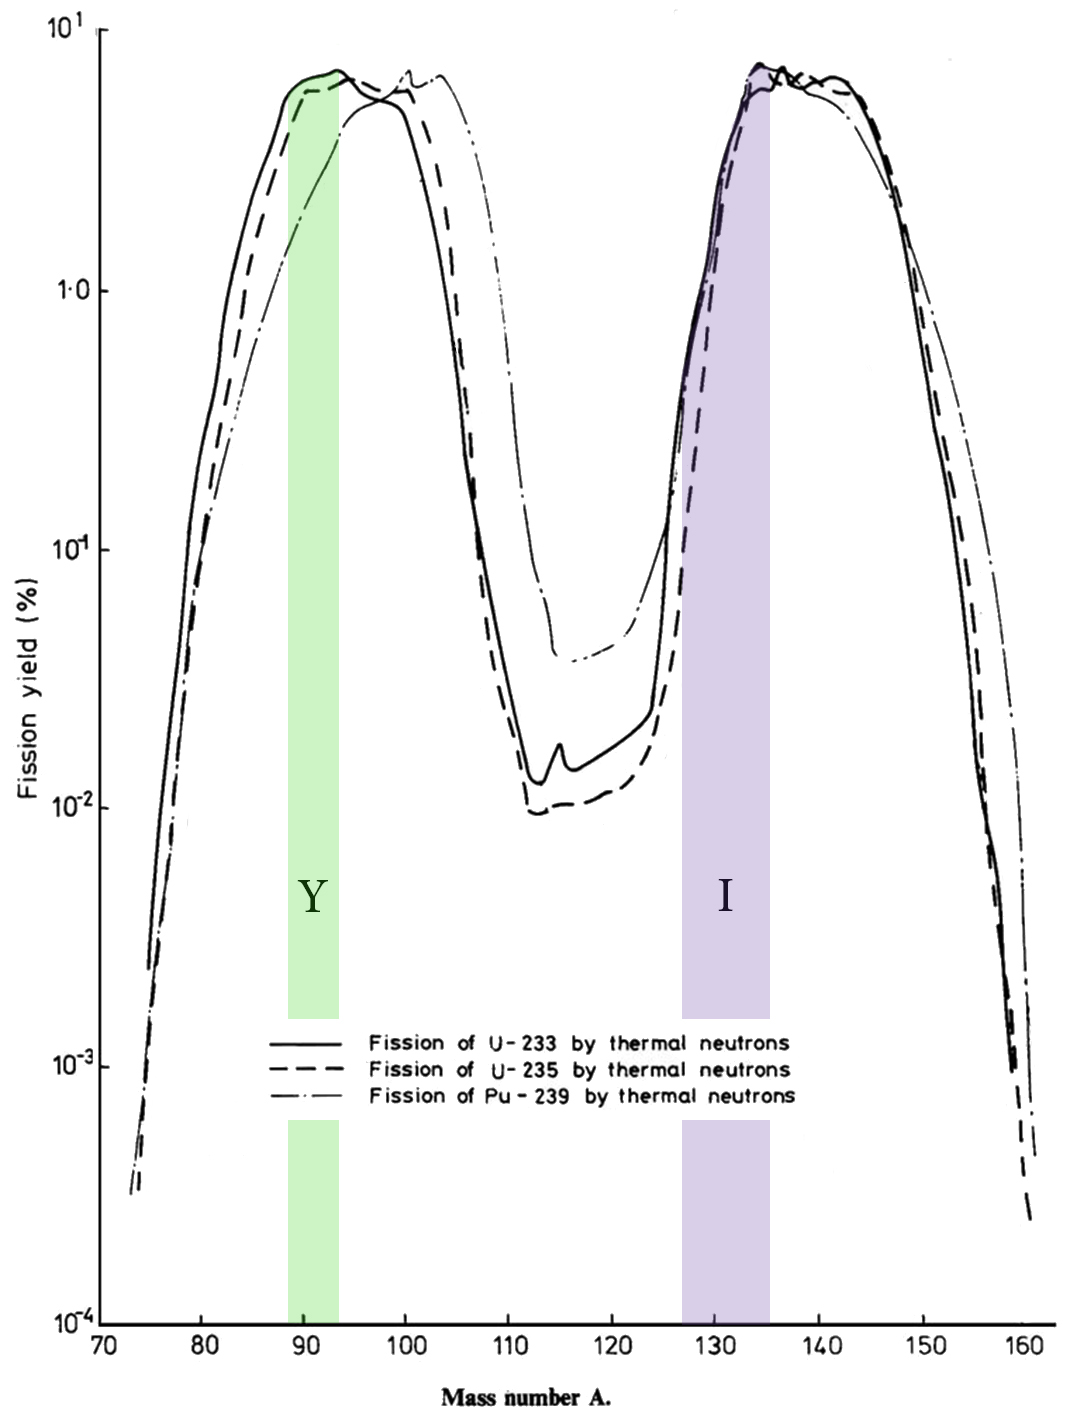
\includegraphics[height=12cm]{images/fissionyield.jpg}
\caption[Plot of the percentage yield of nuclei with a given mass following a fission event. Range of masses corresponding to isotopes of iodine shown in purple and isotopes of yttrium shown in green, based on Equation \ref{eqn:fission}.]{Plot of the percentage yield of nuclei with a given mass following a fission event. Range of masses corresponding to isotopes of iodine shown in purple and isotopes of yttrium shown in green, based on Equation \ref{eqn:fission}. Adapted from \cite{England1992}.}
% M. F. James, R. W. Mills and D. R. Weaver (1991) UKAEA Reports, AEA-TRS-1015, AEA-TRS-1018 
         %  and AEA-TRS-1019.
\label{figure:fissionyield}
\end{figure}

Iodine is an important fission product because it is known to corrode Zr metal. It is part of the Te $\rightarrow$ Cs decay chain, with most isotopes exhibiting half-lives ranging from a few seconds to several days. Select data on Te and I fission yields are presented in Table \ref{table:decaydata_chap1}. In total, the independent yield of I isotopes from U$^{235}$ fission is 11.4\%, while the independent yield of Te isotopes (I precursors) is 18.1\%, with \ch{Te_{52}^{134}} having the highest independent yield of all possible fission products (6.3\%). These particular elements will also usually be paired with Zr and Y fission products, the latter of which is a common phase stabiliser dopant in \zirconia .

\begin{table}[ht!]
\onehalfspacing
\caption{Independent fission product yields and half-lives for the major iodine isotopes and precursors in a thermal neutron reactor. Yields taken from the Joint Evaluated Fission and Fusion File (JEFF 3.3). All isotopes undergo single $\beta$- decay. Metastable states are included.}  \label{table:decaydata_chap1}
\begin{center}
\begin{tabular}{c c c}
\hline
Isotope & Independent Yield (\%) & Half-life \\
\hline
\texorpdfstring{I\textsubscript{131}}{I131} & 0.0029604
 & 8.023 d \cite{I131halflife} \\
\texorpdfstring{Te\textsubscript{132}}{Te132} & 1.5042 & 3.180 d \cite{Te132} \\
\texorpdfstring{I\textsubscript{132}}{I132} & 0.028399  & 2.295 h \cite{Te132} \\
\texorpdfstring{Te\textsubscript{133}}{Te133} & 3.9386 & 12.5 m \cite{khazov2011nuclear} \\
\texorpdfstring{I\textsubscript{133}}{I133} & 0.198194  & 20.87 h \cite{I133} \\
\texorpdfstring{Te\textsubscript{134}}{Te134} & 6.3001 & 41.8 m \cite{Sonzogni2004} \\
\texorpdfstring{I\textsubscript{134}}{I134} & 0.7673 & 52.5 m \cite{Sonzogni2004} \\
\texorpdfstring{Te\textsubscript{135}}{Te135} & 3.4777 & 19.0 s \cite{tellurium135halflife} \\
\texorpdfstring{I\textsubscript{135}}{I135} & 2.4635 & 6.58 h \cite{tellurium135halflife} \\ 
\texorpdfstring{Te\textsubscript{136}}{Te136} & 1.6652 & 17.63  s \cite{Mccutchan2018} \\
\texorpdfstring{I\textsubscript{136}}{I136} & 3.03823 & 83.4 s \cite{Mccutchan2018} \\
\texorpdfstring{Te\textsubscript{137}}{Te137} & 0.48440 & 2.49 s \cite{browne2007nuclear} \\
\texorpdfstring{I\textsubscript{137}}{I137} & 2.7026 & 24.5 s \cite{browne2007nuclear} \\ 
\texorpdfstring{Te\textsubscript{138}}{Te138} & 0.11280 & 1.4 s \cite{chen2017nuclear} \\ 
\texorpdfstring{I\textsubscript{138}}{I138} & 1.2419 & 6.26 s \cite{chen2017nuclear} \\ 
\hline
\end{tabular}
\end{center}
\end{table}

\subsection{Formation of plutonium and minor actinides}

Uranium fuel in LWRs is enriched to contain up to 5\% \ch{U^{235}}, which is a fissile isotope. The rest of the uranium is comprised of the more abundant \ch{U^{238}} which is a \emph{fertile} isotope. Fertile isotopes are not fissioned directly, but can be converted into fissile isotopes through nuclear reactions. In the case of \ch{U^{238}}, the fissile isotope \ch{Pu^{239}} is produced through the following reactions:
\begin{gather}
\ch{U^{238}_{92}} + n^{1}_{0} \xrightarrow[]{absorption} \ch{U^{239}_{92}} \\
\ch{U^{239}_{92}} \xrightarrow[]{\beta-} \ch{Np^{239}_{93}} + e^{-} + \overline{\nu}_{e} \\
\ch{Np^{239}_{92}} \xrightarrow[]{\beta-} \ch{Pu^{239}_{94}} + e^{-} + \overline{\nu}_{e}
\end{gather}
Fresh UO$_{2}$ fuel does not contain any plutonium before irradiation, however, production of \ch{Pu^{239}} during reactor operation is so significant that over 40\% of the energy produced (in a LWR) is from the fission of \ch{Pu^{239}}.2
